
\begin{comment}
\hspace{0.08cm}
\begin{minipage}[b]{0.35\linewidth}
\centering
  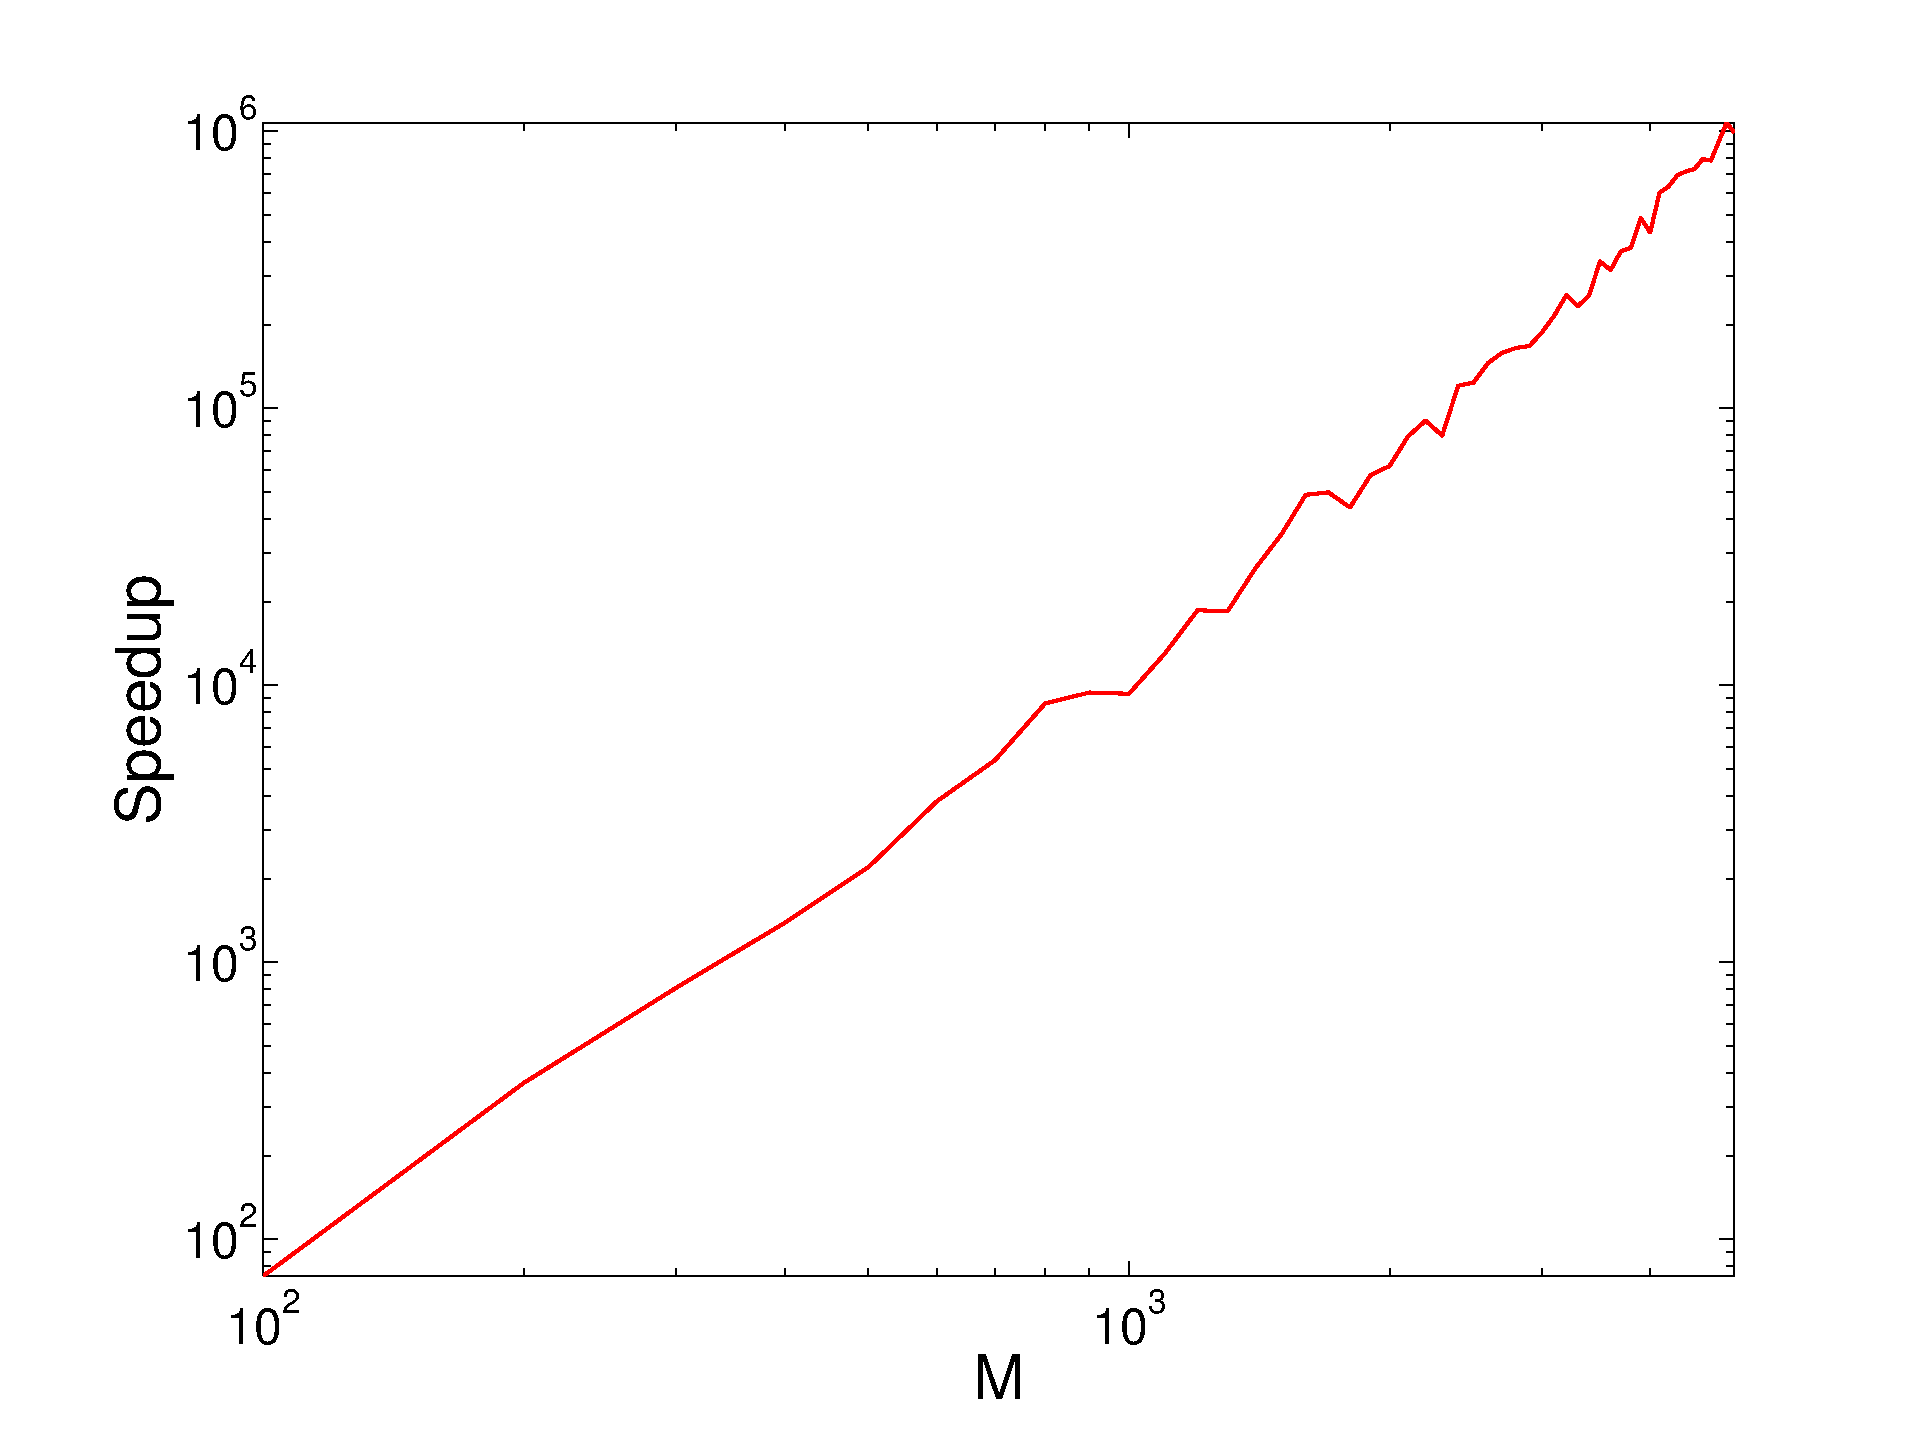
\includegraphics[width=0.7\textwidth,height=0.5\textwidth]{figMInvSpeedUp.eps}
  \vspace{1mm}
  \caption{Speedup of ODC framework prediction on either TGP or GPR while retrieving precomputed matrix inverses as $M$ increases, compared with computing them on test time by KNN scheme (log-log scale)}
  \label{fig:SpeedUp}
\end{minipage}
%\vspace{-10mm}
\end{figure*}
\begin{figure}
\centering
 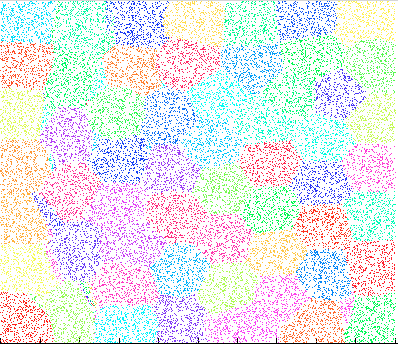
\includegraphics[width=0.25\textwidth,height=0.2\textwidth]{Ekmeans57.png}
 \vspace{4mm}
\caption{Assign and Balance-EKmeans on 300,000 random 2D points, K= 57 (best seen electronically).}
\end{figure}
\end{comment}

Various approximation approaches have  been presented to reduce the computational complexity in the context of GPR. As detailed in \cite{park11}, approximation methods on Gaussian Processes may be categorized into three trends: matrix approximation,
likelihood approximation, and localized regression. The matrix approximation trend is inspired by the observation that the kernel matrix inversion is the major part of the expensive computation, and thus, approximating the matrix by a lower rank version, $M \ll N$\ignore{,   helps reduce the computational demand} (e.g.,  Nystr\"{o}m  Method~\cite{Nystrom01}). While this approach reduces the computational complexity from $O(N^3)$ to $O(N M^2)$ for training, there is no guarantee on the non-negativity of the predictive variance~\cite{Rasmussen:2005}. In the second trend,  likelihood approximation is performed on testing and training examples, given $M$ artificial examples known as inducing inputs, selected from the training set (e.g.,  Deterministic Training Conditional (DTC)~\cite{DTC03}, Full Independent conditional (FIC)~\cite{fic06}, Partial Independent Conditional (PIC)~\cite{pic07}). The drawback of this trend is \ignore{that it deals with }the dilemma of selecting $M$ inducing points, which might be distant from the test point, resulting in a performance decay; see Table~\ref{tab:thcomp} for the complexity of FIC.


\ignore{However, } A third trend, localized regression, is based on the belief that distant observations are almost unrelated\ignore{, and adopted in our work}. The prediction of a test point is achieved through its $M$ nearest points\ignore{ from the training set}. One technique to implement this notion is through decomposing the training points into disjoint clusters during training, where prediction functions are learned for  each of them~\cite{park11}. At test time, the prediction function of the closest
cluster\ignore{, where the test point belongs, } is used to predict the corresponding output. While this method is efficient\ignore{ and adaptive to non-stationary change}, it introduces discontinuity problems on boundaries of the subdomains. Another way to implement local regression is through Mixture of Experts (MoE) as an Ensemble method to make prediction based on computing the final output by combining outputs of local predictors called experts (see a study on MoE methods~\cite{tymoe12}). Examples include Bayesian committee
machine (BCM~\cite{BCM00}), local probabilistic regression (LPR~\cite{LPR08}), mixture of Tree of Gaussian Processes (GPs)~\cite{TreeGPs07}, and
Mixture of GPs~\cite{Rasmussen:2005}. While these approaches overcome the discontinuity problem by the combination mechanism, they suffer from intensive complexity at test time, which limits its applicability in large-scale setting\ignore{. One more computational aspect is that mixture models, as }, e.g., Tree of GPs and Mixture of GPs, involve complicated integration, approximated by computationally expensive sampling or Monte Carlo simulation. 

\ignore{
Park  et al~\citet{park11} proposed an approach for fast computation of GPR with a focus on large spatial data sets. The approach decomposes the domain of a single output regression function into small subdomains, inspired by a domain decomposition  approach for solving  Partial differential Equations (PDEs). It then infers a local regression function for each subdomain. In contrast to prior methods, this approach is easier to parallelize. However, it was mainly based on building consistent boundary value functions between subdomains on  a regular grid. Hence, their approach was evaluated on data of maximum input dimension $2$.}

Park etal.~\cite{park11} proposed a large-scale approach for  GPR by domain decomposition on up to 2D grid on input, where a local regression function is inferred for each subdomain such that they are consistent on boundaries.\ignore{The approach model the problem by solving Partial Differential Equations to maximize consistent prediction on the boundaries of sudomains, defined on a regular grid (upto 2D grid).} This approach obviously lacks a solution to high-dimensional input data because the size of the grid increases exponentially with the dimensions, which limits its applicability\ignore{makes the approach unapplicable in is not applicable to many applications}. More recently,\ignore{  Chalupka et al}~\cite{Chalupka:2013} proposed a Recursive Partitioning Scheme (RPC) to decompose the data into non-overlapping equal-size clusters, and they built a GPR on each cluster\ignore{; we denote this method as Local-RPC}. They showed that this local scheme gives better performance  than FIC~\cite{fic06} and other methods\ignore{ they compared with, in the time regimes as it operates}. However, this partitioning scheme obviously lacks consistency on the boundaries of the partitions and it was restricted to single-output GPR\ignore{, which limits its applicability in structured regression problems, e.g., human pose estimation}. Table~\ref{tab:thcomp} shows the complexity of this scheme denoted by local-RPC for GPR.
 
  
\begin{comment}
Another way to implement local regression is through Mixture of Experts (MoE)  as an Ensemble method to make prediction based on computing the final output by combining outputs of local predictors called experts (see a recent study of MoE approaches \cite{tymoe12}). Examples include Bayesian committee machine (BCM~\cite{BCM00}), local probabilistic regression (LPR~\cite{LPR08}), mixture of Tree of Gaussian Processes (GPs)~\cite{TreeGPs07}, and Mixture of GPs~\cite{Rasmussen:2005}. While these approaches overcome the discontinuity problem by the combination mechanism, they suffer from intensive complexity at test time, which limits its applicability in large-scale setting\ignore{. One more computational aspect is that mixture models, as } (e.g., Tree of GPs and Mixture of GPs, involve complicated integration, which is approximated by sampling or Monte Carlo simulation, that has a big computation cost).


, a common restriction in the prior work
\end{comment}





\begin{comment}
There have been increasing discriminative approaches to tackle pose reconstruction. These approaches were either based on nearest-neighbor schemes \cite{Shakhnarovich, Poppe07} or parametric predictors \cite{Rosales01learningbody, Agarwal06, Sminchisescu:2007}, trained using images of people and their corresponding 3d ground truth pose. A common drawback of these early approaches is that  they do not model the correlation between the outputs. This correlation  was successfully captured in~\cite{Bo:2010} by Twin Gaussian Processes (TGP). Yamada et al~\cite{Yamada:2012}  then proposed a covariance shift approach for TGP  to solve the data bias problem of the training data. In the remaining of this section, we focus on Twin Gaussian Processes work in~\cite{Bo:2010,Yamada:2012}.
\end{comment}

Beyond GPR, we found that local regression was adopted differently in structured regression models like Twin Gaussian Processes (TGP)~\cite{Bo:2010}, and also an data bias version of it, denoted by  IWTGP~\cite{Yamada:2012}.\ignore{ which deal with the data bias problem.In contrast to GPR, these models captures dependency between output dimensions, which leads to  better predictions in the Human 3D pose estimation task. } TGP and IWTGP outperform not only GPR in this task, but also various regression models including Hilbert Schmidt Independence Criterion (HSIC)~\cite{HSIC05}, Kernel Target Alignment (KTA)~\cite{KTA01}, and Weighted-KNN~\cite{Rasmussen:2005}. Both TGP and IWTGP have no closed-form expression for prediction. Hence, the prediction is made by gradient descent on a function that needs to compute the inverse of both the input and output kernel matrices, $O(N^3)$ complexity. Practically,  both approaches have been applied by finding the $M \ll N$ Nearest-Neighbors (NN) of each test  point in~\cite{Bo:2010} and~\cite{Yamada:2012}. The prediction of a test point is  $O(M^3)$ due to the inversion of $M \times M$ input and output kernel Matrices. \ignore{While this NN local regression scheme is one way to tackle the performance problem;} However, NN scheme has three drawbacks: (1) A regression model is computed for each test  point, which results in a scalability  problems in prediction (i.e., Matrix inversions on the NN of each each test point), (2) Number of neighbors might not be large enough to create an accurate prediction model since it is constrained by the first drawback, (3) It is inefficient compared with the other schemes used for GPR. Table~\ref{tab:thcomp} shows the complexity of this NN scheme\ignore{ denoted by NN}.
\ignore{
These drawbacks are overcome as a consequence of the six desirable properties. }